% momentum
\section{Skriðþungi}
Skriðþungi er stærð táknar tregðu hlutars til að breyta hraða og stefnu, sem
almenn regla er skriðþungi táknaður sem vigur stærð. Hins vegar verður einungis
kynntur skriðþungi í einni vídd, sem þýðir að formerki mun tákna stefnu og
stærð skriðþungans verður tölugildið. Í fleiri víddum þarf að nota vigra sem
verður nánar skoðað í áframhaldandi köflum. Fyrst er það skilgreiningin á
skriðþunga
\begin{equation}
	\umomentum = \umass \uspeed
\end{equation}
mikilvægi þessa jöfnu verður útlistað í framtíðarköflum, en til að byrja með
verður skoða þau tilfelli þegar hlutir breyta skriðþunga sínum. Sem er oftast
við árekstra á milli atóma, hluta, kúlna og kassa.

Það eru tvenns konar kerfi sem verða skoðuð, þegar við segjum kerfi er átt við
samansafn af hlutum sem geta verkað á hvort annað. Þegar um lokað kerfi er átt
við að skriðþunginn er varðveittur og hverfur ekki, opið kerfi myndi leyfa massa
að hverfa (þ.e.a.s. hlut) og myndi ekki varðveita skriðþungan%
\footnote{Opin og lokuð kerfi gilda líka um krafta og orku, en hér er einungis
verið að skoða skriðþunga}. Það er líka hægt að tala um samanlagðan skriðþunga
kerfis, þá er skriðþungi hvers hlutar samanlagður og tekið tillit til stefnu
hlutarins.
\[
	\umomentum_\text{heild} = \sum \umomentum = \text{summa allra }\umomentum
\]
þá er táknið $\sum$ notað fyrir samanlagningu á öllum skriðþungum. Það sem gildir
í \emph{lokuðum kerfum} er það skriðþunginn breytist ekki. Sem gefur að
\[
	\umomentum_\text{heild, fyrir} = \umomentum_\text{heild, eftir}
\]
þá er samanlagður skriðþunga fyrir og eftir atvik sá sami.
%
\begin{formalexample}
Tveir bílar lenda í árekstri, bíll A er $\SI{800}{\kg}$ og á 
$\SI{54}{\km\per\hour}$ hraða,
bíll B er $\SI{1500}{\kg}$ og er á $\SI{36}{\km\per\hour}$ hraða. Þegar bílarnir
lenda saman getum áætlað að þeir festast saman og verði einn nýr heildarmassi.
Hver verður hraði nýja massanns eftir árekstur?
\\[4 ex]
Við breytum helstu stærðum í SI-einingar, $\SI{54}{\km\per\hour} 
= \SI{15}{\m\per\s}$ og $\SI{36}{\km\per\hour} = \SI{10}{\m\per\s}$. Síðan 
er stefna bílanna mikilvæg, þar sem bílarnir koma úr \emph{gagnstæðum} 
áttum þýðir að annar hefur neikvæða hreyfistefnu. Ef við áætlum að bíll 
A ferðast í jákvæða stefnu, þá ferðast bíll B í neikvæða stefnu. Þar 
sem við getum fundið heildarskriðþunga fyrir og eftir árekstur, þá er 
heildarskriðþungi fyrir árekstur
\begin{align*}
	\umomentum_\text{heild, fyrir} &= \SI{800}{\kg} \times \SI{15}{\m\per\s}
		+ \SI{1500}{\kg} \times \left( - \SI{10}{\m\per\s} \right) \\
	&= \SI{800}{\kg} \times \SI{15}{\m\per\s}
		- \SI{1500}{\kg} \times \SI{10}{\m\per\s} \\
	&= - \SI{3000}{\N\s}
\end{align*}
þegar bílarnir lenda saman er þá er samanlagður skriðþungi eftir árekstur
\begin{align*}
	\umomentum_\text{heild, eftir} &= 
		\left(\SI{800}{\kg} + \SI{1500}{\kg} \right) \times \uspeed
		\\
	&= 
		\SI{2300}{\kg} \times \uspeed
\end{align*}
þar sem skriðþunginn varðveitist er hægt að segja
\begin{align*}
	\umomentum_\text{heild, fyrir} &= 
		\umomentum_\text{heild, eftir}
		\\
	-\SI{3000}{\N\s} &= 
		\SI{2300}{\kg} \times \uspeed
		\\
	\uspeed &= 
		\frac{-\SI{3000}{\N\s} }{ \SI{2300}{\kg} }
		\\
	&=
		-\SI{1.3}{\m\per\s}
\end{align*}
hér táknar $-\SI{1.3}{\m\per\s}$ að nýi massinn (bíll A og B klesstir saman) stefna
í sömu átt og bíll B, þ.e.a.s. í gagnstæða átt við bíl A.
\end{formalexample}
%
Kraftar og skriðþungi eru nátengdar stærðir, nánar tiltekið, kraftur er afleiða
skriðþunga. Afleiða í stærðfræðilegum skilningi og reyndar almennum líka. Sem
stærð er hægt að tengja skriðþunga og kraft með
\begin{equation}
	\uforce = \frac{\Delta\umomentum}{\Delta\utime}
\end{equation}
s.s. kraftur er jafn stór og breytingin í skriðþunga á tímaeiningu. Sem passar ef
lögmál Newtons eru skoðuð nánar, til að breyta stefnu eða hraða hlutars þarf
að beita krafti. Þá hlýtur að gilda að ef hlutur breytir skriðþunga 
sínum (í stefnu eða stærð) að kraftur hafi verkað á hlutinn, 
annars hefði allt haldist óbreytt.

\subsection{Atlag}
Þegar skriðþungi breytist er hægt að lýsa því sem stærð af krafti og tíma, sem
stærð er atlag
\begin{equation}
	\Delta\umomentum = \uforce \Delta\utime 
\end{equation}
þá er það skriðþungabreyting sem er jafngildi meðalkraftsins margafaldað með
tímanum. Það er líka mikilvægt að gera grein fyrir stefnu skriðþunga, sama og
með krafta, stundum vinna kraftar með eða móti hreyfingu, skriðþungi getur unnið
með og móti hreyfingu hluta.

Sem hluti af þessu, þá er hægt að gera kraft-tíma gröf þar sem flatarmálið undir
grafinu er jafngildi skriðþungans sem hefur verið færður á milli hlutanna. Það
er sjáanlegt á stærðinni $\Delta\umomentum = \uforce \Delta\utime$ að hún svipar
til $\Delta\ulengths = \uspeed \Delta\utime$.
\begin{formalexample}
\begin{wrapfigure}{r}{0.5\textwidth}
	\begin{center}
		\centering
		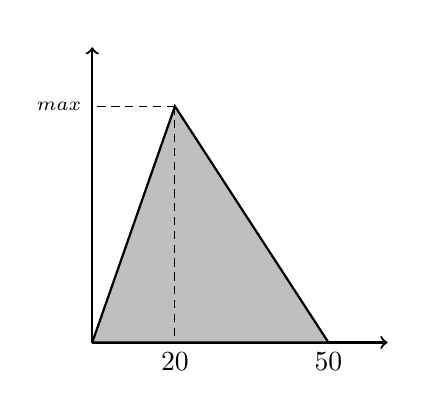
\begin{tikzpicture}[
			bline/.style={thick, fill=lightgray, draw=black},
			axis/.style={thick, draw=black, font=\small},
			scale= 3
		]
			\draw[axis,->] (0,0) -- +(1.25,0) node[right] {$\utime$};
			\draw[axis,->] (0,0) -- +(0,1.25) node[above] {$\uforce$};
			\draw[bline] (0,0) -- ++(0.35, 1) -- ++(0.65, -1) -- ++ (-1, 0);
			%\draw[densely dashed] (0,35,1) -- ++(0,-1) node[right] {$\utime$};
			\draw[draw=black, densely dashed] (0.35, 1) -- +(0,-1) 
				node[below] {$\SI{20}{\ms}$};
			\draw[draw=black, densely dashed] (0.35, 1) -- +(-0.35,0) 
				node[left] {$\uforce_\text{max}$};
			\draw[] (1, 0) 
				node[below] {$\SI{50}{\ms}$};
		\end{tikzpicture}
	\end{center}
\end{wrapfigure}
Bolti lendir á kylfu, áður en boltinn boltinn lendir á kylfunni er hraði boltans
$\SI{10}{\m\per\s}$ og eftir að boltinn lendir kylfunni er hraði boltans er
$8 \uspeedms$ og í gagnstæða átt. 
Það líða $\SI{20}{\ms}$ áður en krafturinn sem boltinn verkar
kylfuna verður stærstur og síðan líða $\SI{30}{\ms}$ þar til kylfan er búin að
verka á boltann. Massi boltans er $\SI{0.10}{\kg}$.
Hvert er hámark kraftsins sem verkar á boltann?
\\[4 ex]
Þar sem við þekkjum hraðan fyrir og eftir kylfuslagið er hægt að finna breytingu í
skriðþunga á þessum $50 \umilli\usec$. Sem gefur
\begin{align*}
	\Delta\umomentum &= \umomentum_\text{eftir} - \umomentum_\text{fyrir} \\
		&= \SI{0.1}{\kg} \times \SI{10}{\m\per\s} 
			- \left( - \SI{0.1}{\kg} \times \SI{8}{\m\per\s} \right) \\
		&= \SI{0.9}{\N\s}
\end{align*}
og allt flatarmálið undir grafinu er jafn stórt og þessi stærð, flatarmálið er gefið
sem
\begin{align*}
	\Delta\umomentum &= \frac{1}{2} \uforce_\text{max} \Delta\utime_1
		+ \frac{1}{2} \uforce_\text{max} \Delta\utime_2 \\
	\SI{0.9}{\N\s} &= 
		\frac{1}{2} \times \uforce_\text{max} \times \SI{0.020}{\s}
		+ \frac{1}{2} \times \uforce_\text{max} \times \SI{0.030}{\s} \\
	\SI{0.9}{\N\s} &=
		\left(
			\frac{1}{2} \times  \SI{0.020}{\s}
			+ \frac{1}{2} \times \SI{0.030}{\s} 
		\right) 
		\times 
		\uforce_\text{max} \\
	\SI{0.9}{\N\s} &=
		\SI{0.025}{\s} \times \uforce_\text{max} \\
	\uforce_\text{max} &=
		\frac{ \SI{0.9}{\N\s} }{ \SI{0.025}{\s} }
		= \SI{36}{\N}
\end{align*}
sem er hámarkið á kraftinum sem hefur verkað á boltann er því í beinu samræmi við hversu
lengi og hversu stór skriðþungabreytingin er.
\end{formalexample}
